\chapter[ETH BiodivX in XPrize Rainforest Finals]{Robotic Biodiversity Assessments: ETH BiodivX's Robots in the XPRIZE Rainforest Finals}
\label{ch:XP}
	
	\author{Christian~Geckeler\authorrefmark{1,2}, Georg~Strunck\authorrefmark{3}, Salua~Hamaza\authorrefmark{3}, and Stefano~Mintchev\authorrefmark{1,2}}
	\affil{Environmental Robotics Laboratory, Dep. of Environmental Systems Science, ETH Zurich, 8092 Zurich, Switzerland}
	\affil{Swiss Federal Institute for Forest, Snow and Landscape Research (WSL), 8903 Birmensdorf, Switzerland}
	\affil{Biomorphic Intelligence Lab, Faculty of Aerospace Engineering, TU Delft, 2629HS Delft, The Netherlands}
	\corresp{Corresponding author: Christian~Geckeler (email: cgeckeler@ethz.ch).}
	\authornote{This work was supported by the Swiss National Science Foundation through the Eccellenza under grant number 186865. It was further supported by the Rütli-Stiftung, the ETH Foundation, the XPRIZE Foundation, and the Alana Foundation via the participation of the authors in the XPRIZE Rainforest competition. Salua Hamaza's work was supported by NWO VENI grant 20308.
	}
	
	
	% 150-250 words
	\begin{abstract}
		Abstract Here
	\end{abstract}
	
	\begin{IEEEkeywords}
		% Enter key words or phrases in alphabetical order, separated by
		% commas. Using the \textit{IEEE Thesaurus} can help you find the best
		% standardized keywords to fit your article. Use the \underline{\href{https://www.ieee.org/publications/services/thesaurus.html}{thesaurus
				% access request form}} for free access to the \textit{IEEE Thesaurus}.
	\end{IEEEkeywords}
	
	%\IEEEspecialpapernotice{(Invited Paper)}
	
	\maketitle
	
	\section{INTRODUCTION}
    \label{sec:introduction}
	\IEEEPARstart{T}{ropical} 
 rainforests are among the most biodiverse ecosystems on Earth, home to millions of species of plants, animals, fungi, and microorganisms, many of which remain undiscovered. This biodiversity is vital for maintaining ecosystems that benefit the planet, such as carbon sequestration, water cycling, and oxygen production, which are essential for regulating the global climate and supporting life on Earth \cite{lewis2015increasing}\cite{stork2007tropical}.
%Adding to that, rainforests act as reservoirs of genetic diversity, offering immense potential for biotechnological and pharmaceutical innovations. Many of the world’s medicines, including treatments for cancer, heart disease, and infections, have been derived from rainforest species. By studying this biodiversity, scientists can uncover new compounds with medicinal properties, leading to potential breakthroughs in healthcare \cite{mendelsohn1995value}.

Despite the global significance of rainforests, much of their biodiversity remains unexplored and poorly understood \cite{stork2007tropical}. These ecosystems are home to an estimated half of the world’s terrestial vertebrate species, many of which have yet to be identified or studied in detail \cite{Pillay2022}. Even as new species are discovered regularly, there is still limited knowledge about their roles within the ecosystem, their interactions with other species, and their responses to environmental changes. This lack of information is particularly concerning given the accelerating threats of deforestation and climate change, which may drive species to extinction before they can be studied. Especially the yet undiscovered species often are the most endangered ones, underpinning the necessity of more thorough research of the rainforests \cite{georgLiu2022}.
The threat from humans through deforestation, habitat fragmentation, and climate change endangers not only the species living there but also the ecosystem's overall health. The urgently needed research helps to understand the impacts of human activities on these ecosystems and to develop effective conservation strategies. Studying rainforest biodiversity aids in understanding the intricate relationships between species and their environment, guiding restoration efforts and laying the foundation for sustainable land use.

To gain faster and better access to rainforest research, the XPRIZE Rainforest competition aims towards largely autonomous solutions to survey the biodiversity of a given rainforest area in only 24 hours of sampling.
This paper introduces the procedures and designs of the multiple solutions that have been developed by the ETH BIODIVX team throughout the competition. 

After introducing the entire system in \autoref{sec:system_overview} ...
	
	%% For half-page, 1-column figure
	% \begin{figure}[!t] % or [!htp]
		% \centering
		% 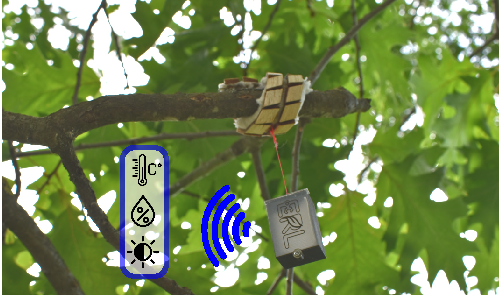
\includegraphics[width=1\columnwidth]{figures/figure1-overview.pdf}
		% \caption{interesting caption here}
		% \label{fig1_overview_intro}
		% \end{figure}
	
	%% For full page, 2 column figure (in coreldraw should be 2 page)
	% \begin{figure*}[!t] % or [!htp]
		% \centering
		% 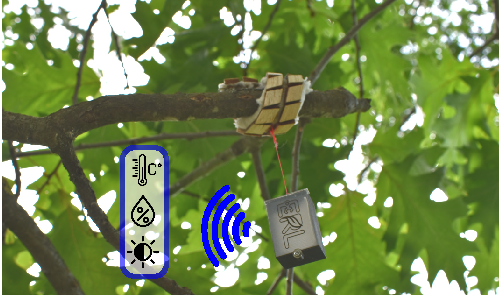
\includegraphics[scale=1]{figures/figure1-overview.pdf}
		% \caption{interesting caption here}
		% \label{fig1_overview_intro}
		% \end{figure*}
	

    % already eDNA sampling withe eProbe, more autonomous biodiv. assessment etc. etc
    % background of contest
    % transition from singapore

 
    \section{COMPETITION OVERVIEW}
    The main goal of the XPrize Rainforest competition is to generate the most insights into the biodiversity of 100 ha of rainforest within the given time. During the first 24 hours, the teams can collect data from the base camp, outside of the buffer zone, XX m from the competition area. The following 48 hours are available to analyze the data and formulate insights from them. From a robotics perspective, there are 4 main challenges: coverage, time, safety, and the type of data to be collected. Collecting data from 100 ha of rainforest is not trivial, especially if physical samples are collected which do not permit flying hundreds of meters above the canopy. At this point, maintaining a stable communication connection for control and feedback becomes problematic. Likewise, having only 24 hours within which to collect all data requires efficient collection with limited human resources. Solutions should be robust, reliable and safe; crashing a drone or failing to retrieve a sensor would result in deducted points. For comprehensive insights, different types of data not conventionally collected with robots should be collected: surface eDNA, water eDNA, insect samples, or acoustic recordings.
% time, (=> automation + efficient collection)
    % coverage, covering full 100 ha (automaiton, communication)
    %safety
    % maybe collected data types (multi-modalitiy, insect traps, water/surface edna etc)
    %autonomy vs teleoperaiton
    To address these issues, we focus on automation, communication, and diverse data sources. Through autonomous sample collection data collection efficiency and coverage is improved. Maintaining communication with the drone enables further coverage for manual data collection, and improves safety for autonomous operations. 

    In general the strategy was to minimize risk to avoid unnecessary point deductions and to maximize species detections through diverse complimentary data sources. These include close-up image of vegetation and insects, eDNA collected from surfaces and water, bioacoustic recordings, and physical insect specimens.    
    %sampling strategy/data collection approach (minimze risk, collect mulitple different types of data
    
	\section{SYSTEM OVERVIEW}
    \label{sec:system_overview}
    % The different data modalities require different collection methods. For collecting the surface eDNA< 
    
    Since all equipment must be portable and transported by the participants into the field, the hardware was kept to a minimum while still allowing for redundancies in case of failures. Therefore, the main workhorse was the DJI M300, which can complete different tasks by exchanging modular payloads. Adding the DJI Zenmuse P1 RGB camera allows for mapping of the area, the DJI Zenmuse H20 for close-up image capture, our custom winch payload for either surface eDNA sampling or water eDNA sampling, and a mount for deploying and retrieving the raft. By simply exchanging the payload, most necessary robotic tasks in the field can be achieved with the same drone. In total, there were two DJI M300, a DJI Mavic 3 Pro, and a DJI Mavic 3 Classic. The DJI Mavic drones were used for close-up images, videography, scouting, and providing an additional reference viewpoint (e.g. for raft deployment).

	\section{MAPPING}

%TODO: Figure: competition area map (react/matic) with DEM height profile difference
    %- dimensions (e.g. to furthest point, buffer, etc
    %- maybe some nice stats (e.g. how many images, how long to process, etc
 
 %    - mapping (for eDNA) ⇒ extraction of maps

%necessary for location scouting (rafts), for elevation planning eprobe, water scouting
% also used for tree segmentation ?
% first quick and dirty map

Both for information and to later conduct autonomous operations, the first task for the competition was to create a map. To this end, data from the whole area is captured, and then a parallel approach was used to first process the data quickly to get a lower-resolution map for basic canopy height. Using this map, the next data capturing missions can be planned while the higher resolution and more accurate map is processed. Once this more accurate map is processed, the increased accuracy can be used for more challenging missions, such as flying closer to the treetop canopy or with reduced visibility such as at night where manual visual safety checks are more challenging.
Since the exact coordinates of the 100 ha area were published 24 hours in advance, photogrammetry flights were planned in advance to cover the area. UgCS from SPH Engineering \cite{Engineering} was used to plan for the photogrammetry missions, with the following settings: 80\% horizontal and vertical overlap and a flight altitude of XXm. The DJI Zenmuse P1 was used to capture images, which, with the chosen flight height, results in a ground sample distance (GSD) of 1.56 cm/pixel. The altitude was chosen as a trade-off between time needed for data capture, time needed for processing, and the resulting resolution. The full mapping took XX(2?) flights/min, resulting in XX images.

To facilitate downstream tasks which require the RGB orthomosaic and DEM, an initial result, even with reduced quality, is essential. To this end, PIX4DReact, a Structure from Motion (SfM) photogrammetry tool for first responders, was used to generate the initial DEM and orthomasic. Processing took XX min, and the results can be seen in Fig. XX, Including data capture and processing, the initial full RGB orthomosaic and DEM were available within two hours. 

After the initial PIX4DReact processing, another higher resolution but more computationally intensive reconstruction was performed, using PIX4Dmatic. This processing took XX mm and is shown in Fig. XX.
While qualitatively judging the orthomosaics visually, differences are difficult to determine, the DEM demonstrates significant differences, with deviations of up to XXm (Figure XX2) between the two. Figure XX shows the height profile for a sample transect of the two maps and the corresponding differences. For this reason, the initial map was used as an initial estimate with enhanced safety margins to compensate.
	
	\section{COMMUNICATION}

% Figure: layout of the nodes during the 1.5km sampling (e.g distance of the mast to the raft, to the drone, etc)
    %- inset with picture of mast, the communication node on raft (check biodiv report/existing figures
%  - Back-up Communication (=> mast + raft)
% - beyond range sampling

One of the largest robotic challenges in surveying the 100 Ha is communication. If the systems are teleoperated, a continuous communication link is needed to control and receive feedback from the robot. If the robot is fully autonomous, then it is also possible to move beyond the communication range of the ground station and pilot, under the assumption that safety mechanisms will ensure flight and operational safety under all eventualities.
Indeed, for the mapping flights, the connection between the remote and UAV was lost for the last third of the area, during this time the UAV was flying and capturing data fully autonomously, with no redundant communication link.
Since lowering a probe into the vegetation is more risky than capturing images from above, for eDNA collection it was decided to utilize a back-up communication channel which would directly connect with the onboard computer. This communication link would provide feedback to the pilot on the current sampling status as well as trigger or abort commands.

Looking at Figure XX, the competition area is 100 ha, but longer than it is wide, so, under consideration of the 300 m wide buffer zone, from the pilot's position to the furthest point within the competition area is 1.5 km. Despite impressive ranges on the spec sheets, the actual range for both the stock DJI Antenna and similar communication devices is much less (advertised as up to 14 km under ideal conditions, in our field conditions measured up to 500m). This is mainly due to the environment, occlusions, and the drone position. Since the pilot's position is not elevated, there can be quite some trees between the pilot's position and the UAV, which already reduces the range due to the Fresnel effect. Since the drone is less than 20m from the caonpy for surface eDNA sampling, this effect is even more prevalent than if it was flying at higher altitudes, for mapping for instance. Rainforests, with high humidity, dense foliage, and potentially also fog, present a particularly challenging case.

Therefore, a node-based 2.4GHz mesh network (Rajant Breadcrumb) was chosen as a communication medium. The mesh network approach removes the need to reliably maintain a single monolithic connection, instead multiple nodes can extend the range while also providing redundancy. 2.4 GHz provides ample data bandwidth and was shown during testing to also maintain sufficient range. 
During the finals testing, a total of four such wireless nodes were utilized to collect eDNA samples beyond the range of the stock DJI remote. At the base station, one module on top of a 7m rollable mast (Rollatube) enabled the base-station laptop connection over WiFi for feedback and control. A second node was located on the communication raft (Section/Figure XX) which was placed XX m into the competition area, thus providing an intermediate node for the UAVs. The last nodes are located on each of the two DJI M300 UAVs. One drone carried out the sampling, and the other acted as a relay drone, positioned between the communication raft and the the sampling drone. The nodes on the UAVs enable both connection of the onboard computer on the UAV with the ground station and extension of the mesh network. Most of the eDNA samplings (Figure XX) were done in the lower third of the competition area, where the fixed communication raft was sufficient to maintain connection. For sampling the furthest distance from the basestation (1.5km), both UAVs were used, with the relay drone hovering stationary at XX m between the communication raft and the sampling UAV, maintaining the communication connection for the full 1.5km. 

The laptop at the ground station then could monitor the status of the payload and trigger the sampling procedure. Due to safety considerations, this was done manually, but of course can also be conducted autonomously.


    \section{AUTONOMOUS SURFACE EDNA COLLECTION}

%TODO Figure: nice image from the videos of the probe going into the vegetation, user interface on the RC, collected probe

    % Collection mechanism
    In \cite{Kirchgeorg2024} the eProbe is first described, a payload system used for collecting surface eDNA using a swab which is lowered and raised into the vegetation, as used by the ETH BiodivX team in the XPrize rainforest semi-finals in Singapore. For the XPrize Rainforest Finals, an upgraded version of the same system is used. 
    For enhanced usability, the winch payload system utilizes the DJI PSDK interface provided by DJI for payload development. This allows a single USB-C connection from the drone to both power the payload and provide communication between the onboard computer and the RC. Once the payload is plugged in, a custom widget on the default DJI piloting app appears, allowing full control of the payload without having to switch the interface. Simple status feedback, such as the length of the tether and force on the winch is also shown through a debug menu. For more comprehensive logging and debug, a separate connection to the onboard computer can be made and the payload controlled and feedback monitored through the command-line. 
    
% descirbe major changes ()

    The points sampled are shown in Figure XX. A risk-averse sampling strategy was chose for the competition. Most of the surface eDNA samples were taken in the lower third of the competition area, within the standard remote range to ensure safety and stable communication. Fully autonomous sampling was also done for these sites for the same reason. For full coverage of the competition area three points were sampled in the last third of the competition area, at a range of up to 1.5km from the base station. For safety, these samples were taken under supervised autonomy, where the drone flew to the location autonomously, but every lowering of the probe was manually commanded, after which the probe lowered and raised autonomously. The entire process was commanded and supervised through the back-up communication link. 

    %% different autonomy modes? ie full/partial/probe/etc supervised?  

    To ensure the safety of the drone and environment, several layers of redundant safety procedures were employed. First, for all samples a communication link was maintained so that feedback can be monitored and commands can be sent to the payload, either through the standard default drone RC, or through the back-up communication link. For the lowering and raising of the probe, the same algorithm as in \cite{} was used to avoid entanglements. If an entanglement is detected, the user is notified with a warning message. The user can then choose to engage a manual brake, which locks the winch spool, and then proceed to raise the drone, which can exert more force to free the probe. The load cell on the winch continues to provide force measurements and can indicate how hard the probe is being pulled. If this is unsuccessful, a hot-wire cutting mechanism can sever the tether and ensure safety of the drone, at the expense of losing a probe and leaving it in the environment. While this was also incorporated into the fully autonomous workflow, it was not used for the competition since since leaving objects in the environment is penalized and a continuous communication link is maintained.

    % - Autonomous/Automated eDNA collection state machine (JFC)
    % - safety mechanisms/layers
    % - DSM + sensors
    % - waypoint + conservative buffer
    % - cutting mechanism ( backup relay)

    \section{WATER EDNA COLLECTION}

    %TODO: Figure: image from above with the pump pumping water 
    Water eDNA can be collected with the same, payload mechanism, simply replacing the probe with custom developed water pump. The pump has a separate power source and microcontroller, with a WiFi module which connects to the onboard computer on the UAV. Even with manual piloting the distance to the water surface is difficult to estimate, so the pump was set to automatically engage the pump once in the water. For this, the center of gravity of the pump is adjusted so that once the pump is in the water it tilts, an embedded IMU detects this tilt and starts the pump, also stopping the winch from lowering. Once the sampling time has elapsed, the pump stops pumping and sends the raise command to the winch.

    \section{RAFT}
    \sh{TODO} and \cm{TODO}
\textbf{This section should be 1 full page with figure.}

As can be understood from \autoref{sec:introduction}, researching the biodiversity of inaccessible rainforest regions is a crucial step towards understanding the impact of global climate factors and local pollution and deforestation on Earth's natural habitats. As it is estimated that $70-90$\% of life is found in the tree canopy \cite{butler2019} it only makes sense to also focus on that part of the rainforest for research. 

A drone-deployable canopy raft offers a new tool in the field of tropical rainforest exploration and research. Traditionally, canopy research, which focuses on the biodiversity and ecological processes occurring in the uppermost layers of forests, has been limited by difficult access to these heights. Techniques to reach the canopy layers, such as rope climbing \cite{dial1994description}\cite{picart2014cafotrop}, cranes \cite{Wright2010}, or large manned aerial platforms like blimps \cite{Aberlenc2007} have been used but come with high costs, logistical complexity, and limited manoeuvrability. This has created a pressing need for lightweight, autonomous solutions that can quickly access difficult-to-reach canopies without disrupting the fragile ecosystem.

Our design of a drone-deployable canopy raft (seen in \autoref{fig:canopy_raft} aims to solve these challenges. By using aerial robots, the raft can be deployed precisely and efficiently onto the canopy from above, allowing scientists to explore otherwise inaccessible regions. The raft is constructed from lightweight materials designed to distribute weight evenly across the treetops, ensuring minimal impact on the delicate ecosystem. Once deployed, the raft provides a platform to collect samples and use instruments like light traps for observations. Additionally, the raft has been designed in a modular way, allowing it to be outfitted with new modular components, such as solar panels for energy independence and other equipment for collecting environmental data over extended periods.

\begin{figure}
    \centering
    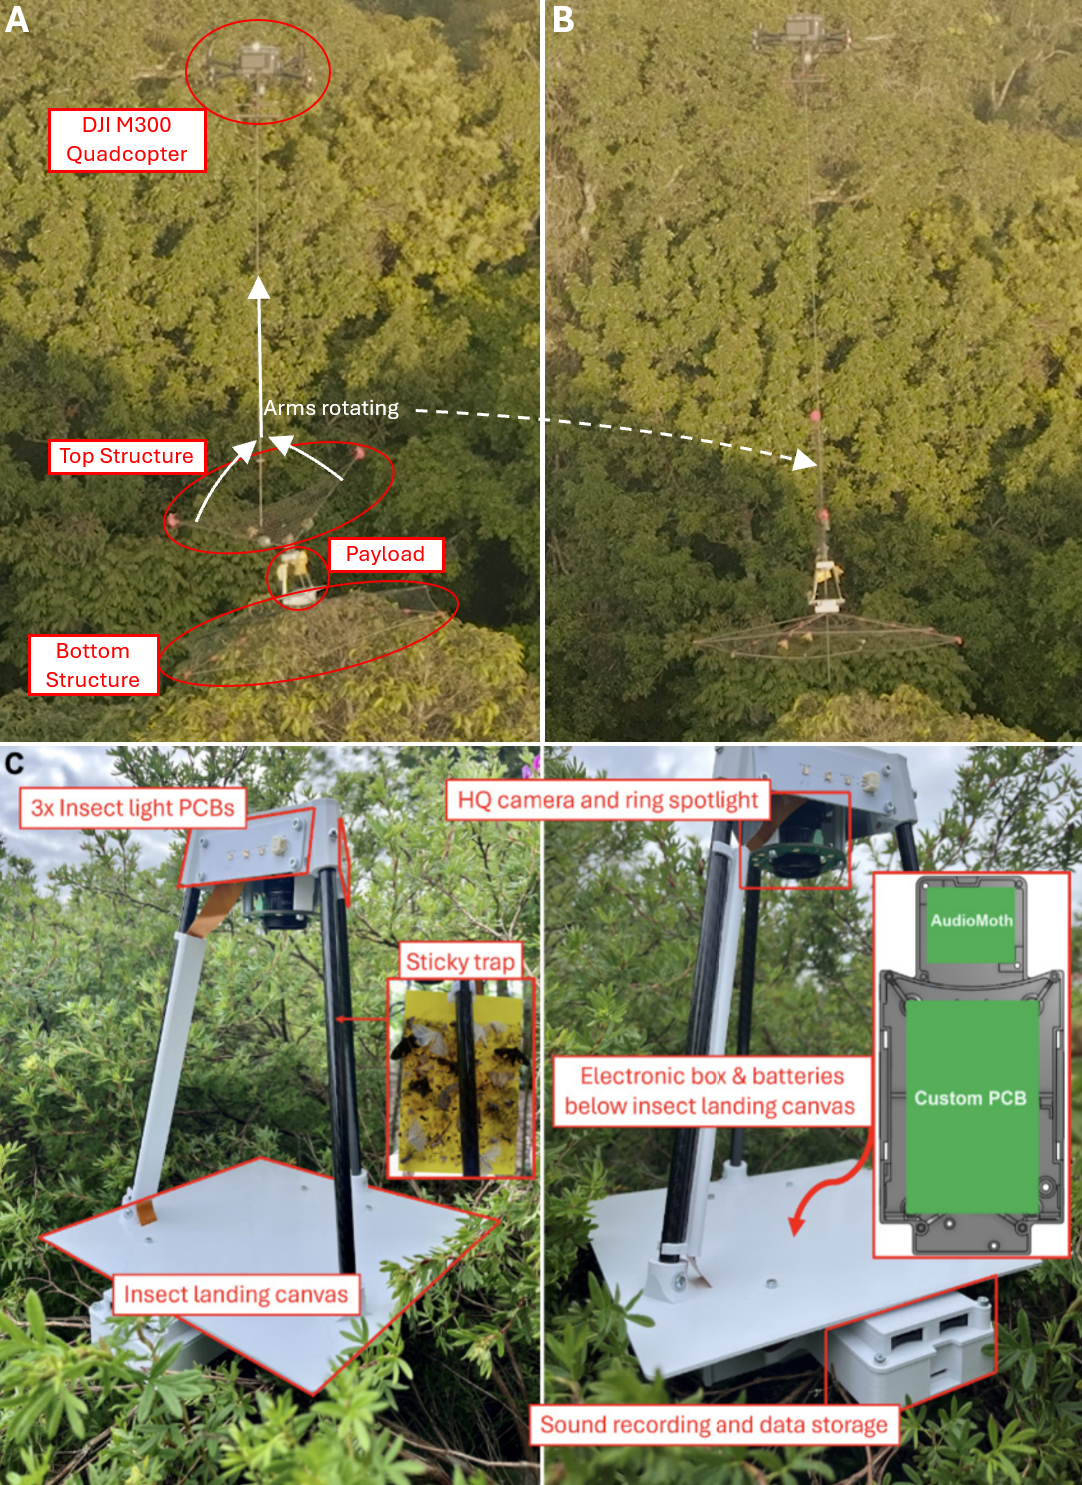
\includegraphics[width=0.8\linewidth]{figures/canopy_raft.png}
    \caption{The canopy raft being retrieved by quadcopter (A-B) and its payload for the xPrize rainforest finals competition in detail.}
    \label{fig:canopy_raft}
\end{figure}

    \subsection{STRUCTURE}
    % comm raft
    % other raft
    \sh{TODO}
The main objective of the canopy raft is to deliver a sensor payload to the tree tops. To do so a retrievable hexagonal platform of $2$ [m] diameter was designed to support the load of both the structure and payload on the upper canopy layer (see bottom structure in \autoref{fig:canopy_raft}A). The raft has been sized to fit the maximum payload of the carrying quadcopter, a DJI M300, of $2.7$ [$kg$]. According to Halle et al. \cite{halle2000}, the average canopy structure can support about $1.7$ [$kg/m^{2}$], leading to a minimum requirement of $1.6$ [$m^2$] of contact area with the canopy for the maximum payload. For convenience of manufacturing an area of $2.6$ [$m^2$] has been chosen, including a safety factor of $1.6$ [$-$]. The beams are made out of $10/8$ [$mm$] carbon rods, centre pieces printed in carbon fibre-reinforced high-temperature nylon, and supporting netting made of polyethylene wires.

For retrieval, a top structure is connected to the top of the payload. It holds at its base a passive hook releasement system for deployment and a wide triangle sail made of polyethene netting. This sail is easy to catch with a treble hook connected to the quadcopter on a $3$ [$m$] wire. 

Both for deployment and retrieval the PTS4 payload release mechanism with a downward-facing camera was used to both allow for a visual on the raft and as an emergency release. This mechanism, including the carrying wires and frame adds up to a weight of less than $200$ [$g$].

The connection to the payload is made with a top-down universal M5 bolt-nut configuration, ensuring a modular, fast-to-set-up design with easily exchangeable payloads.

The top and bottom structures add up to about $500$ [$g$] in total and the design quickly assembles without additional tools. The disassembled state fits in a regular $120$[cm] poster tube for easy transportation and protection in rugged situations.

    \subsection{DEPLOYMENT}
    \sh{TODO}
The deployment of the canopy raft takes place in 3 main steps - the pre-deployment, deployment and retrieval.

During \textbf{pre-deployment}, a fitting location has been (currently manually) scouted for with a DJI Mavic3. For the raft ideally a flat, dense tree trop for safest deployment is being chosen, while angled deployments of up to $30$ [$deg$] have been found stable. The scouting can be automated if a 3D scan of the research area is available. Flat sections can then identified with available Python scripts \footnote{https://github.com/georg-strunck/LOcalize\_Flat\_Topped\_Trees\_Yonder}.

\textbf{Deployment} itself is done by taking off with the carrying drone, connecting the passive hook to the raft and flying (autonomously) to the preplanned GPS waypoint. There the drone slowly lowers until the weight and with it the passive hook are released.

For \textbf{retrieval} a treble fishing hook is attached to the drone, which then flies to the canopy raft location. Once there, it is being lowered in a step-wise fashion, moving laterally to the catching sail at each step. Pink high visibility markers have been added to the design, allowing better judgement (and possible future automation) of the orientation and location of the raft with respect to the drone. Once connected the raft will be pulled up vertically to a safe travelling altitude and then returned to the base station.

    \subsection{PAYLOAD}
    %comm raft


    %sticky trap + camera + audio +...
    \cm{TODO}

    \section{RESULTS}
    
%TODO Figure: large figure which shows the overlay for all the different sampling points (surface, water, close-up images)
    % Figure: sampling sites /different methods
        % - close-up image collection for tree segmentation

    % Figure: Graph Species/method

    % Figure% MOTU DNA collected/ something

    % Figure: Graph Time / Method


    \section{DISCUSSION} 

    \subsection{AUTONOMY VS TELEOPERATION}
    % wide gap between research prototypes and field ready models
    % custom-built platforms with complicated software stacks that few but those who developed it can get to run
    % however, for the solutions to have an impact, they should be usable with minimal training and debugging.
    % xprize unique opprotunity, since only 24 hours and 100Ha, should have high TRL platform, with also the goal that solutions are later used to monitoir biodiversity in the ecosystems.
    % this means simple systems which are robust, user-friendly and efficient at collecting the data
    % fundamentally there are two sides of a scale for operating the systems, and solutions can be somewhere on this scale between full autonomy and total teleoperation. Full autonomy is user-friendly since the user no longer has to directly control the robot, but the user is limited in control input (e.g. mapping missions, out-of-range), where as for full teleoperation the user is in full control, but also has to manually continuously control the robot. This is a gradual scale where there are also intermediate states, for instance supervised autonomy where the robot operates almost fully autonomously but requires intermittent high-level user input for tasks, or partial autonomy where the user still controls the robot but certain tasks are automated, such as the surface eDNA sampling for the eProbe, which has an autonomous control loop, only requiring the user to press the start button. 
    % Full autonomy is difficult to  achieve due to the high safety requirements, all eventualities must be aconuted for, and user-input is also not available for things such as sampling site locations, where an experts opinion is invaluable and can be difficult to automate.
    %Full teleoperation is not user-friendly and not scalalble, since the pilot must control every aspect of the mission.
    % An ideal solution lies somewhere in the middle, where certain parts of the mission are fully automated, but still allow user-input, for instance choosing where to sample, autonomously flying to the sampling location, and then autonomously sampling (as for the surface edNA sampling. A pilot is still supervising the operation and can provide input or adjust the mission as needed, but low level tasks such as the sampling and flying to the location are automated.
    % For maximum scalability, as much as possible should be automaed, for example
    % For the surface eDNA collection at 1.5km, a back-up communication channel was established with quite some effort to initiate and supervise the process for safety reasons. With further developments in the solution and the appropriate legal certifications, this sampling can also be performed fully autonomously, requiring only the planning of the mission where to sample.
    % Scalability?

    \subsection{VEGETATION DENSITY AS AN ASSET}
    % probe + raft
    Usually in the field of robotics, dense and unordered vegetation is treated as an obstacle that should be circumvented or avoided. However, it is also possible to leverage the density and unstructured nature of foliage as an asset. In order to collect eDNA, the collector material on the eProbe requires contact with the environment, with a positive correlation between the number, duration and force of the contacts. Since the eProbe is passive without additional directional actuators, it does not actively target specific surfaces to contact, instead it relies on chance and sufficient repetitions to collect eDNA. In this case, dense vegetation is beneficial since there is an increased likelihood of contacts. The design of the eProbe minimizes the risk of entanglements, and thus denser jumbles of branches and leaves transform from risky regions to be avoided to areas that should be sampled due to the higher likelihood of contact.
    Similarly for canopy rafts, denser regions of the canopy represent areas that can safely sustain higher loads and are thus preferred and sought out over sparser areas when placing the raft. 
    

    %future work     
 
	\section{CONCLUSION}
	The conclusion goes here.
	
	\section*{ACKNOWLEDGMENT}
	\cg{TODO}, \sh{TODO}, \cm{TODO}
	
% 	\bibliographystyle{bibtex/IEEEtran}
% 	\bibliography{bibtex/references.bib,bibtex/control,bibtex/references2}
	
	
% 	\vfill\pagebreak
	
% \end{document}
